\chapter{Requisiti Progetto}
\section{Archittetura PX4}
PX4 rappresenta un software open source specializzato nel controllo di veicoli unmanned, offrendo ai programmatori una vasta gamma di strumenti e un supporto completo sia a livello software che hardware. Nella figura \ref{fig:PX4_Arch}, si presenta un quadro panoramico ad alto livello del controllore di volo implementato in PX4:
\begin{figure}[h]
    \centering
    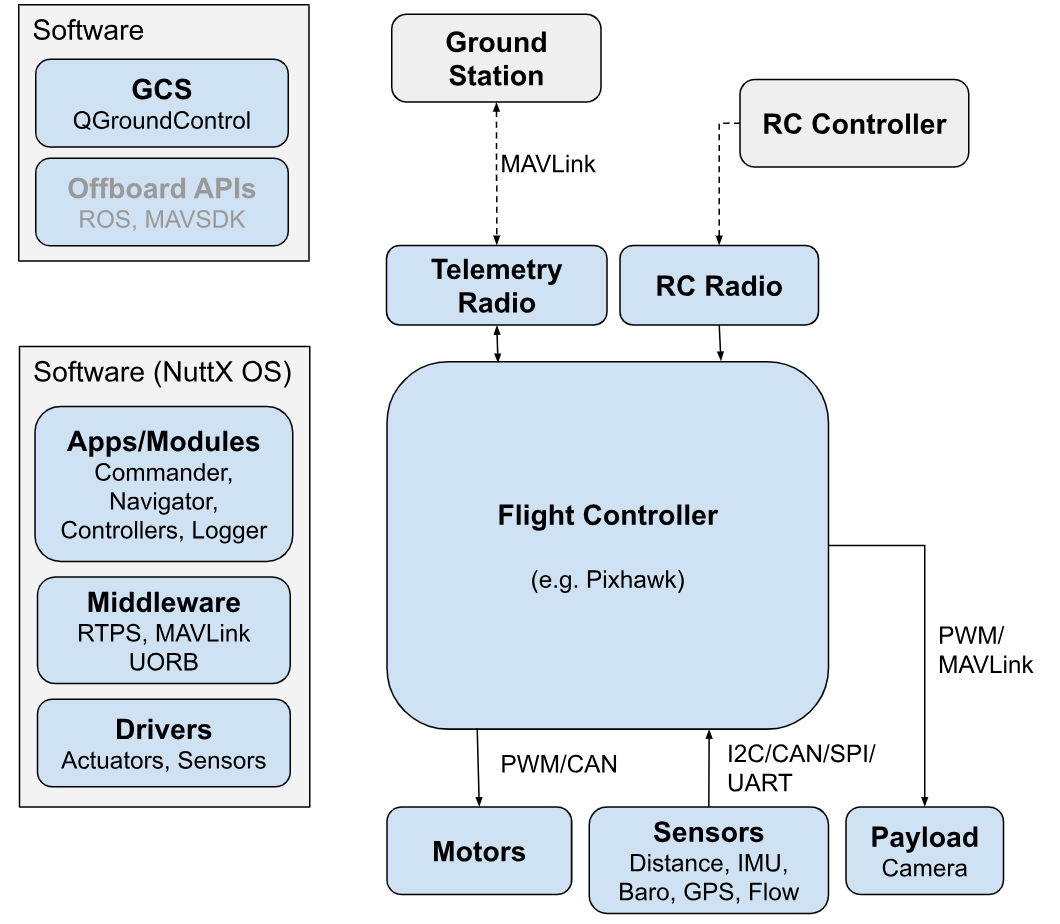
\includegraphics[width=0.7\linewidth]{PX4_Architettura.png}
    \caption{Architettura di alto livello del controllore di volo in PX4}
    \label{fig:PX4_Arch}
\end{figure}
\\
Dal lato hardware, la configurazione comprende diversi componenti chiave:
\begin{itemize}
    \item Controllore di volo (PixHawk): Esegue lo stack PX4, fornendo un'interfaccia fondamentale per la gestione complessiva del drone.
    \item ESC (Electronic Speed Control): Questi circuiti regolano la velocità e la direzione di rotazione dei motori, collegandosi alle uscite PWM del controller.
    \item Sensori: Connessi al controller tramite bus I2C o UART, forniscono dati essenziali per la navigazione e il controllo.
    \item Fotocamera: Collegata tramite canale PWM o protocollo MAVLink, consente la raccolta di dati visivi e può essere integrata nelle attività di controllo del drone.
    \item RC Controller: Necessario per il controllo manuale remoto attraverso un Joypad.
\end{itemize}
Sul fronte software, la configurazione include:
\begin{itemize}
    \item QGroundControl: Utilizzato come stazione di controllo da un computer host, fornisce un'interfaccia utente per monitorare e comandare il drone.
    \item Stack di volo PX4: Eseguito sul controllore di volo, comprende moduli di comunicazione, driver e middleware. La sua architettura di alto livello è rappresentata nella Figura 
\end{itemize}

